% !TeX spellcheck = en_US
\documentclass[10pt,a4paper,notitlepage,twocolumn]{article}
\usepackage[utf8]{inputenc}
\usepackage{amsmath}
\usepackage{amsfonts}
\usepackage{amssymb}
\usepackage{graphicx}
\usepackage{listings}
\usepackage{wasysym}
\usepackage[hidelinks]{hyperref}
% \usepackage{float}

\DeclareMathOperator*{\argmin}{arg\,min}

%opening
\title{Continuum Normalization using Synthetic Spectra}
\author{Christian Brock \footnote{Dresden Gönnsdorf Observatory}}
\date{February 2019}
\begin{document}

\setlength{\parindent}{0pt} 
\setlength{\parskip}{4pt} 

\maketitle

\begin{abstract}
	For a quantitative analysis of measured spectra, an accurate and reproducible continuum normalization is essential.
	We show how such a normalization can be implemented using the data points of synthetic spectra as reference.
\end{abstract}

\section{Introduction}

For an amateur project observing the $H\alpha$ emission of an accretion disc around Algol ($\beta$ Persei) \cite{Bitnar2017}, we needed to compare the observed spectra against synthetic spectra of an B8V star showing no emissions.

As the intensity of the emissions is below ten percent of the continuum, we needed a good SNR\footnote{signal to noise ratio} and a very accurate continuum normalization.

The ESO Midas documentation \cite{EsoMidas} Volume B states:
\begin{quote}
	A frequently used procedure, alternative to the correction for the chromatic response, is to normalise the continuum to unity by dividing the observed spectrum by a smooth approximation of its continuum.
\end{quote}

There are several approaches to solve this problem:
\begin{itemize} % \itemsep -8pt
\item Richards \cite{Richards1993} p.\ 259, table 2 and Liebisch \cite{Liebisch2018} use linear approximations of data points at predefined wavelengths, usually one to the left and one to the right of an observed absorption line.
\item The software tool Visual Spec \cite{DesnouxVSpecTutorial} allows the user to interactively enter continuum points with the mouse and then uses a "softened" spline to approximate the continuum.
\item ESO Midas \cite{EsoMidas} also allows to enter continuum points interactively, it then uses spline fits by default (see \cite{SablowskiSchanne2018} p.\ 502).
\end{itemize}

All interactive methods have the following drawbacks. They
\begin{itemize} % \itemsep -8pt
	\item depend on expert knowledge of the user,
	\item are not reproducible,
	\item require a continuum to be present, which is a problem with cold stars or spectra of a narrow wavelength region around a broad absorption line,
	\item cannot be used for any but small observation campaigns.
\end{itemize}

In this paper we argue that all this drawbacks can be overcome using data points from synthetic spectra of the observed stars.
For this we need to apply some transformations to the synthetic spectrum.
\begin{itemize} % \itemsep -8pt
	\item For the {\bf redshift}\footnote{This should be called {\em wavelength correction} as it could also be a blueshift. However, for readability we will stick with the incorrect name {\em redshift}.}  of the synthetic spectrum to fit the observed spectrum we need to consider the radial velocity of the observed star.
	\item The {\bf spectral resolution} of the synthetic spectrum needs to be changed to match the observed spectrum.
\end{itemize}

We implemented the normalization using the Python programming language, especially the numpy \cite{numpy} and astropy \cite{astropy:2013} \cite{astropy:2018} packages.

We are aware, that there are other normalization methods, e.g.\ using recorded standard stars. A good overview can be found by Trypsteen and Walker \cite{TrypsteenWalker2017} pp.\ 70-75.

\section{Methods}

\subsection{Preparation of the synthetic spectrum}

\paragraph{Where to get one}
For this work we did not calculate our own spectra.
For enthusiasts we recommend having a look at iSpec \cite{BlancoCuaresmaSoubiranHeiter2014} (see figure \ref{fig:iSpec}).
\begin{figure}[ht]
	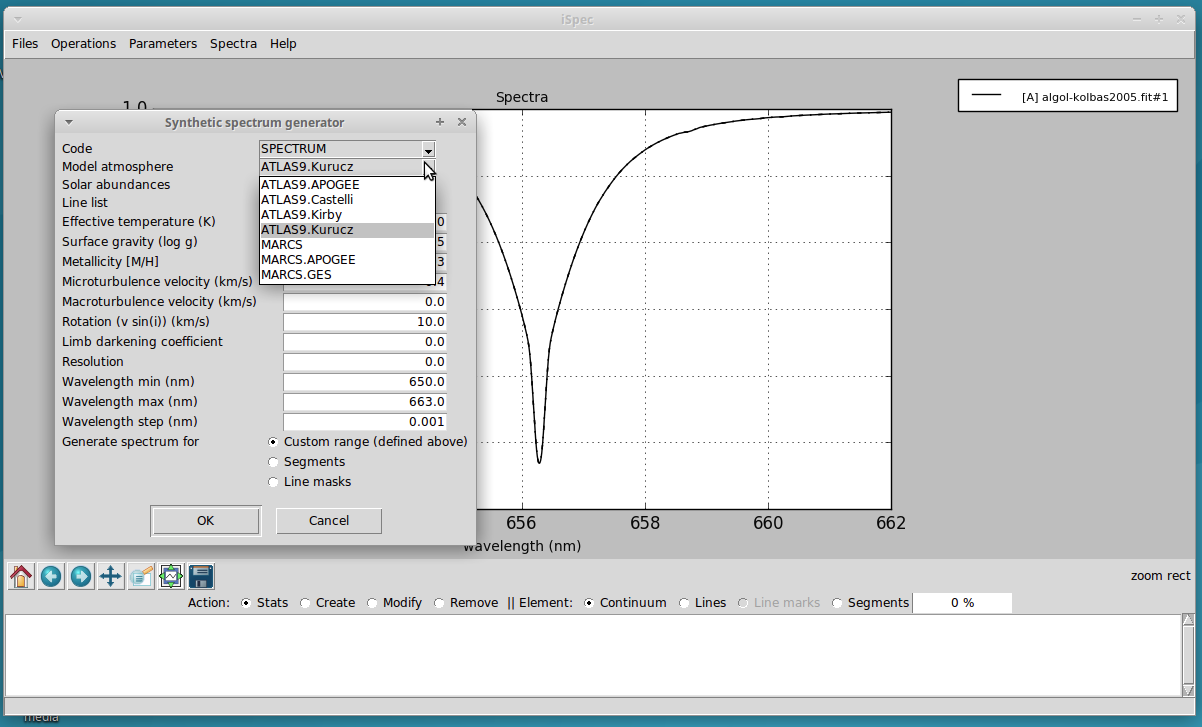
\includegraphics[width=\columnwidth]{img/iSpec.png}
	\caption{iSpec combines several spectral models under a common interface \cite{BlancoCuaresmaSoubiranHeiter2014}}
	\label{fig:iSpec}
\end{figure}

For our work we used the "The POLLUX Database of Stellar Spectra" \cite{Pollux2010}. It supports more spectral models (see figure \ref{fig:pollux}) and does not require the installation of additional software.
\begin{figure}[ht]
	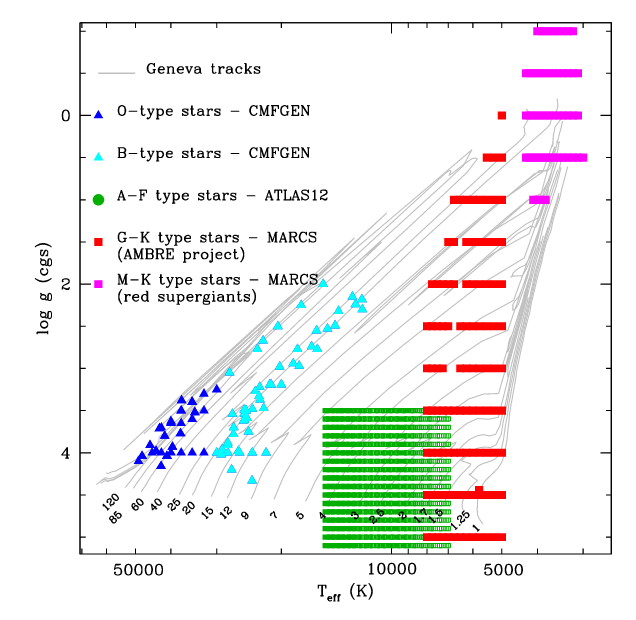
\includegraphics[width=\columnwidth]{img/pollux_models.png}
	\caption{Spectral models used by "The POLLUX Database of Stellar Spectra" \cite{Pollux2010}}
	\label{fig:pollux}
\end{figure}

To choose a spectrum one needs at least the effective temperature, surface gravity, metallicity and rotational velocity of the target star.
Such parameters can be found in the Simbad \cite{Simbad} database.



\paragraph{Applying redshift}

For the redshift of the synthetic spectrum to fit the one of the observed spectrum we need to consider the radial velocity of the observed star.
For ordinary stars this value can be found in online databases such as Simdad \cite{Simbad}.
For binary or hierarchical star systems one has to model the orbits of all system components \cite{Gerlach2015}.
This by itself is a major project and will be subject of a future publication.
At the time of this paper we know of no standard software to implement such models.

Here we assume that the radial velocity of the target star in relation to the sun $v_{* \rightarrow \sun}$ is known.
We can then calculate the radial velocity of the star in relation to the earthbound observer $v_{* \rightarrow \earth}$:
\begin{equation}
	\label{eq:rv}
	v_{* \rightarrow \earth} = v_{* \rightarrow \sun} - v_{\earth \rightarrow \sun}
\end{equation}
$v_{\earth \rightarrow \sun}$ is the heliocentric or barycentric correction -- the velocity component toward the target star caused by earth moving around the sun (see figure \ref*{algol_bary}).
It can be calculated using the \texttt{astropy.\-coordinates.\-SkyCoord.\-radial\_\-velocity\_\-correction} method.

\begin{figure}[ht]
	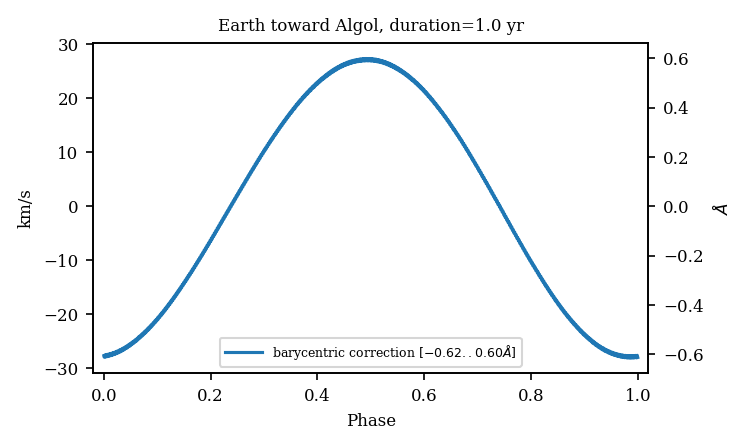
\includegraphics[width=\columnwidth]{img/algol_bary.png}
	\caption{Barycentric correction for the Algol system during a single year}
	\label{algol_bary}
\end{figure}

Having the stars radial velocity toward earth we can then calculate the redshift:
\begin{equation}
	\label{eq:dl}
	\Delta\lambda_{rv} = \overline{\lambda} \frac{v_{* \rightarrow \earth}}{c}
\end{equation}
with $\overline{\lambda}$ as center wavelength of the observed spectrum and $c$ the speed of light.

It is also possible to derive the redshift from the measured data itself.
One can measure the wavelength difference of absorption line minima between the observed and synthetic spectra.

\paragraph{Modifying spectral resolution}
We also need to apply the resolution of the observed spectrum $RESOL$ to the synthetic spectrum.
We do this by convolution of the synthetic spectrum with a Gaussian kernel having a standard deviation of:
\begin{equation}
	\sigma = \frac{\overline{\lambda}}{2.3548\ RESOL}
\end{equation}
$2.3548$ is the the FWHM\footnote{full width half maximum} of the standard Gaussian. See Sablowski and Schanne \cite{SablowskiSchanne2018} p.\ 320 for an explanation how spectral resolution is defined.

Convolution can be done with the \verb|astropy.convolution.convolve| method applying a \verb|astropy.convolution.Gaussian1DKernel| to the spectrum.

\subsection{Continuum approximation}

For the continuum approximation, the "smooth approximation" as explained in chapter 1, we assume that our continuum can be modeled by a polynomial $p_n$ of a given degree $n$ with additional Gaussian noise.
\begin{equation}
	\label{eq:cont_model}
	cont = p_n + \epsilon
\end{equation}

\paragraph{Masking}
Before we continue one additional thought:
We may want to exclude some wavelength regions of the observed spectrum when we know in advance that the observed spectrum does differ significantly from the synthetic one.
In our Algol example we wanted to measure emission features in the center of the $H\alpha$ line.
This exclusion can be done by masking that regions.

Additionally, excluding high slope regions makes the approximation more robust against redshift and resolution errors. 


\paragraph{Getting the polynomial}
Having all in place we are able to calculate a smoothed approximation of the continuum:
\begin{equation}
	\label{eq:cont_approx}
	cont_{approx} = \argmin_{p_n} \sum_{\lambda} \left( p_n - \frac{observed}{synth} \right)^2
\end{equation}
We sum over the wavelengths of the unmasked data points.
Fitting can be done with the \verb|numpy.polyfit| method.

\paragraph{What degree?}
The polynomial degree depends on the fitted wavelength range and on properties of the spectrograph.
This is demonstrated in figure \ref{four_spectra}.
In general, as the number of data points vastly exceeds the polynomial degree, the approximation is very robust against oversampling.
In the Algol project we usually use $n=5$.
If unsure one can use the AIC\footnote{Akaike information criterion} \cite{Akaike1974} to choose the degree that best fits the data.

\begin{figure}[ht]
	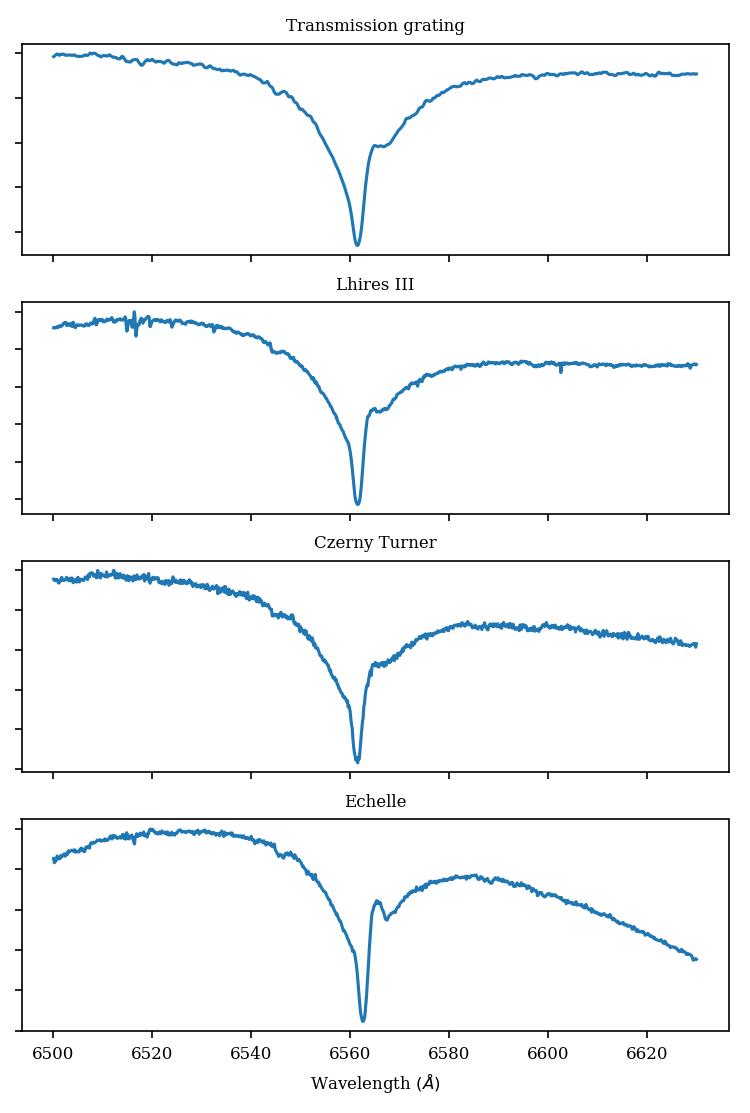
\includegraphics[width=\columnwidth]{img/four_spectra_big_4x1.png}
	\caption{$H\alpha$ measured by four different spectrographs. One can see how polynomials of different degree may be required to fit the different spectra. The Echelle requires a degree of $n=5$ while the others only need a $3$. Many thanks to Uwe Zurmühl (transmission grating), Bernd Bitnar (Lhires III) and Ulrich Waldschläger for the spectra.}
	\label{four_spectra}
\end{figure}


\paragraph{About SNR}
Equation \ref{eq:cont_approx} minimizes the noise term $\epsilon$ in equation \ref{eq:cont_model}.
We see that our continuum approximation minimizes that noise, i.e.\ maximizes the SNR.
The $\argmin$ argument is called residual. It can be used to calculate the SNR:
\begin{equation}
	residual = \sum_N \left( p_n - \frac{observed}{synth} \right)^2
\end{equation}
$N$ are the data points used for the approximation, the measured points of the observed spectrum (not removed by masking).
\begin{equation}
	\sigma_\epsilon = \sqrt{ \frac{residual}{\|N\|}}
\end{equation}
\begin{equation}
	\label{eq:snr}
	SNR = 1 / \sigma_\epsilon
\end{equation}
The residual is one of the results of \verb|numpy.polyfit|.
$\|N\|$ donates the number of data points used for the approximation.\footnote{The 1 in the nominator of equation \ref{eq:snr} is actually misleading. It should be replaced by the maximum or the average of the observed spectrum.}

\subsection{Normalization}
The normalized spectrum can then be written as:
\begin{equation}
	spec_{norm} = \frac{observed}{cont_{approx}}
\end{equation}

Figure \ref*{normalize_howto} shows the entire process.

\begin{figure}[ht]
	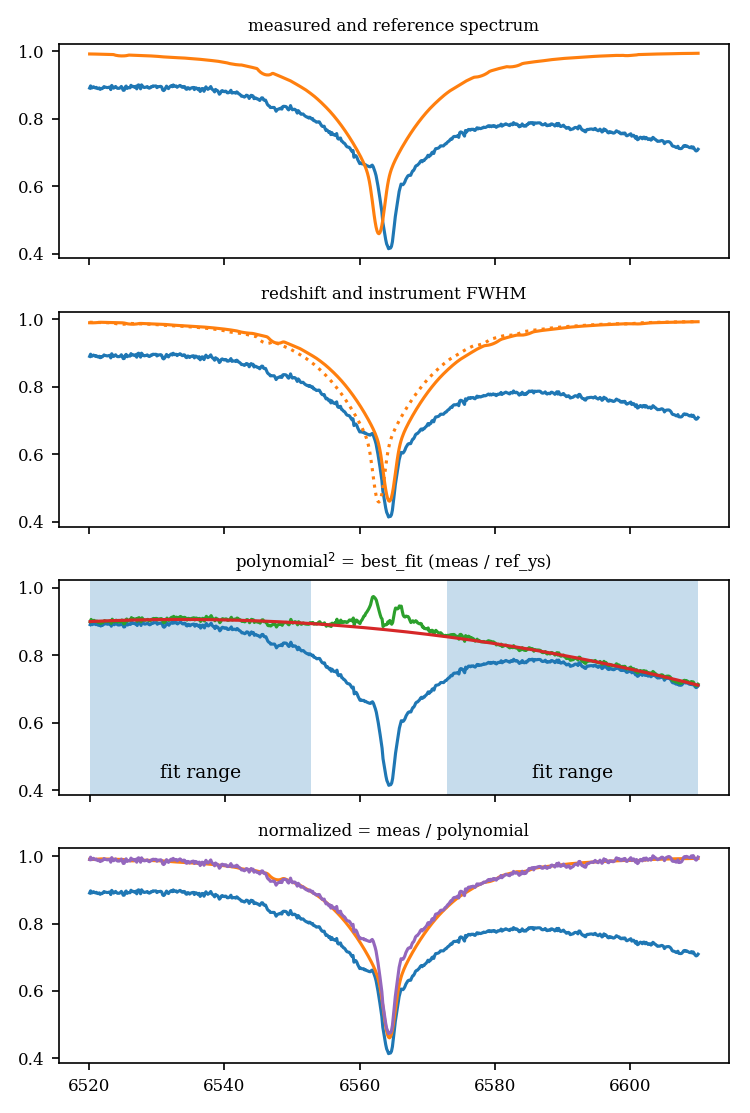
\includegraphics[width=\columnwidth]{img/normalize_howto_4x1.png}
	\caption{The entire normalization process containing, redshift, convolution with the FWHM of the instrument resolution, calculation of the best fitting polynomial and finally the normalization. The fit, the red curve in the third plot, is calculated in the blue area -- the line center, the white area, is masked.}
	\label{normalize_howto}
\end{figure}


\section{Conclusions}

We have shown that data points of synthetic spectra can be used for continuum normalization. The approach is very accurate, reproducible, robust against parameter variations and can be used in an automatic pipeline of observation campaigns.
It is preferable to manual procedures implemented in many tools.

We further displayed that the least square fit of the continuum approximation optimizes SNR.

\paragraph{Software}
The author implemented the entire normalization as Python command line tool.
It can be downloaded undo \url{https://pypi.org/project/algol-reduction/}.

\paragraph{Acknowledgments}
The author would like to acknowledge the help received from the spectroscopic community, especially his local Dresden group and the people running the Dresden Gönnsdorf Observatory. Special thanks goes to Bernd Bitnar, Enrico Gerlach, Thomas Hunger, Josefine Liebisch and Ulrich Waldschläger (in alphabetical order)

\bibliographystyle{plain}
\bibliography{all}

\section*{About the author}
% \includegraphics[width=\columnwidth]{img/cwb.png}
During daytime Christian Brock programs algorithms to optimize cellular networks.
At night he attends to visitors at the Dresden Gönnsdorf Observatory, mentors students, does some visual observations himself and cooperates in the Dresden spectroscopy group.

\end{document}
